\documentclass[a4paper]{article}

\setlength{\parindent}{0pt}
\setlength{\parskip}{1em}

\pagestyle{headings}

\usepackage{amssymb}
\usepackage{amsmath}
\usepackage{amsthm}
\usepackage{mathtools}
\usepackage{graphicx}
\usepackage{hyperref}
\usepackage{color}
\usepackage{microtype}
\usepackage{tikz}
\usepackage{pgfplots}
\usepackage{pgfplotstable}

\newcommand{\N}{\mathbb{N}}
\newcommand{\Q}{\mathbb{Q}}
\newcommand{\Z}{\mathbb{Z}}
\newcommand{\R}{\mathbb{R}}
\newcommand{\C}{\mathbb{C}}
\newcommand{\D}{\mathcal{D}}
\renewcommand{\S}{\mathcal{S}}
\renewcommand{\P}{\mathbb{P}}
\newcommand{\F}{\mathbb{F}}
\newcommand{\E}{\mathbb{E}}
\newcommand{\bra}{\langle}
\newcommand{\ket}{\rangle}


\graphicspath{{Image/}}

\hypersetup{
    colorlinks=true,
    linktoc=all,
    linkcolor=blue
}

\theoremstyle{definition}
\newtheorem*{axiom}{Axiom}
\newtheorem*{claim}{Claim}
\newtheorem*{conv}{Convention}
\newtheorem*{coro}{Corollary}
\newtheorem*{defi}{Definition}
\newtheorem*{eg}{Example}
\newtheorem*{lemma}{Lemma}
\newtheorem*{notation}{Notation}
\newtheorem*{prob}{Problem}
\newtheorem*{post}{Postulate}
\newtheorem*{prop}{Proposition}
\newtheorem*{rem}{Remark}
\newtheorem*{thm}{Theorem}

\DeclareMathOperator{\vdiv}{div}
\DeclareMathOperator{\grad}{grad}
\DeclareMathOperator{\curl}{curl}
\DeclareMathOperator{\Ann}{Ann}
\DeclareMathOperator{\Fit}{Fit}
\DeclareMathOperator{\Diag}{Diag}
\DeclareMathOperator{\tr}{tr}
\DeclareMathOperator{\im}{im}
\DeclareMathOperator{\Mat}{Mat}
\DeclareMathOperator{\Log}{Log}
\DeclareMathOperator{\Isom}{Isom}
\DeclareMathOperator{\Mesh}{Mesh}
\DeclareMathOperator{\Sym}{Sym}
\DeclareMathOperator{\Aut}{Aut}
\DeclareMathOperator{\cosech}{cosech}
\DeclareMathOperator{\Card}{Card}
\DeclareMathOperator{\Gal}{Gal}


\setcounter{section}{-1}

\begin{document}

\title{Stochastic Financial Models}

\maketitle

\newpage

\tableofcontents

\newpage

\section{Motivation}
An investor needs a certain quantity of a share (or currency, good, etc), however, not right now ($t=0$) but at a later time ($t=1$). The price of the share $S(w)$ at time $t=1$ is random, but already today one has to make calculation with it so there is risk. For example, 500USD $\approx$ 370 GBP today. What about in one year?

Possible solution: purchase a financial derivative such as:\\
$\bullet$ forward contract: right and obligation to buy a share at time $t=1$ for a strike price $K$ specified at time $t=0$. Its value at time $t=1$ should be $H(w) = S(w) - K$ is positive if $S(w) > K$, and negative i	f $S(w) < K$;\\
$\bullet$ call-option: the right, but no obligation, to do the same thing as above. Its value at $t=1$ should be $H(w) = (S(w)-K)^+$, i.e. $S(w)-K$ if that is positive, and 0 otherwise (no obligation to exercise the option).

One question: what is the fair price for such a derivative?

1) Classical approach: Regard payoff $H(w)$ as lottery, modelled by a random variable on $(\Omega,F,\P)$, where $\P$ is the 'objective probability measure'.\\
a) very classical: fair price = expected discounted payoff = $\E[\frac{H}{1+r}]$, where $r$ is the interest rate for funds/loans from $t=0$ to $t=1$.\\
Assumption: both interest rates are the same for large investors.\\
b) classical: subjective assessment of the risk (by the seller of $H$) by utility functions.

2) More modern approach: suppose the primary risk (share) can only be traded in $t=0$ and $t=1$.\\
Hedging strategy: $\theta^1$ = number of shares held between $t=0$ and $t=1$;\\
$\theta^0$ = balance on bank account with interest rate $r$.\\
Here we allow $\theta^1$ to be either positive or negative (i.e. allow short-selling).

Price at $t=0$: $\theta^0+\theta^1 \pi^1 = V_0$, where $\pi^1$ is the price of one share at $t=0$.\\
The value of this portfolio at $t=1$: $\theta^0(1+r) + \theta^1 S(w) = V(w)$.

Requirement: value of derivative = value of strategy, $H(w) = V(w)$ for all $w \in \Omega$.

For example, for forward contract: $S(w)-K = V(w) = \theta^0(1+r)+\theta^1 S(w)$, we should choose $\theta^1 = 1,\theta^0=\frac{-K}{1+r}$, so $V_0 = \pi^1 - \frac{K}{1+r}$. The seller of $H$ has no risk if he uses this strategy(?).

Even more, $\pi(H)=V_0$ is the unique fair price for the forward contract. Any other price $\tilde{\pi} \neq V_0$ would lead to \emph{arbitrage}: a riskless opportunity to make profit, which should be excluded). For example, if $\tilde{\pi} > V_0$, at $t=0$ sell forward for $\tilde{\pi}$ and buy the strategy for $V_0$. Then in $t=1$ deliver share and repay the loan. We gain a pure profit at $t=1$: $(\tilde{\pi}-V_0) (1+r)>0$, i.e. arbitrage.

Questions: how to characterize arbitrage-free market? How to determine fair prices of options and derivatives?

\newpage

\section{Utility and mean variance}

The market is interaction of agents trading goods. Individual agents have preferences over different contingent(?) claims (=specified random payment). Agents' preferences are expressed by an expected utility representation. $Y$ is preferred to $X$ means $\E[U(X)] \leq \E[U(Y)]$ with utility function $U: \R \to [-\infty,\infty)$ which is non-decreasing. We assume $U$ to be concave, in the sense that we expect agents to dislike risks.

\begin{defi} 
(1.1) A function $U:\R \to [-\infty,\infty)$ is \emph{concave} if $\forall p \in [0,1]$, $pU(x) + (1-p) U(y) \leq U(px+(1-p)y)$. Let $P(U) = \{x: U(x)>-\infty\}$.
\end{defi}

\begin{rem} (1.2)\\
(a) If $U$ is concave, then $-U$ is convex;\\
(b) Jensen's inequality: $\E[U(X)] \leq U(\E[X])$. Note that this means if an agent is offered a contingent claim $X$ (a random variable) and a certain payment $\E[X]$, then the agent prefers the certain payment. This shows that concave utility functions implies risk-aversion.\\
If $U$ is linear, the agent is risk neutral as it doesn't matter between the two forms of payment; if $U$ is convex then the agent will be risk friendly, since $X$ is now preferred to $\E[X]$.\\
(c) If $U(x) = -\infty$ then the outcome $x$ is completely unacceptable.
\end{rem}

\begin{eg}(1.3)\\
Some example of utility functions:\\
(1) $U(x) = -e^{-\gamma x}$, $\gamma>0$ is the constant absolute risk aversion (CARA) utility.\\
(2) 
\begin{equation*}
\begin{aligned}
U(x) = \left\{\begin{array}{ll}
\frac{x^{1-R}}{1-R} & x \geq 0\\
-\infty & x < 0
\end{array}
\right.
\end{aligned}
\end{equation*}
where $R>0$, $r \neq 1$ is the constant relative risk aversion (CRRA) utility.\\
(3) 
\begin{equation*}
\begin{aligned}
U(x) = \left\{\begin{array}{ll}
\log x & x > 0\\
-\infty & x \leq 0
\end{array}
\right.
\end{aligned}
\end{equation*}
is the logarithmic utility.\\
(4) $U(x) = \min(x,\alpha x)$, $\alpha \in [0,1)$.\\
(5) $U(x) = -\frac{1}{2} x^2 + \alpha x$, $\alpha \geq 0$. This is concave, but not increasing.\\
(6) $U_1$, $U_2$ are utilities, $\alpha_1,\alpha_2 \geq 0$, then $\alpha_1 U_1 + \alpha_2 U_2$ is also a utility.\\
(7) If $\{U_\lambda,\lambda \in \Lambda\}$ is a family of utilities, then $U(x) = \inf_{\lambda \in \Lambda} U_\lambda (x)$ is a utility.
\end{eg}

\begin{prop} (1.4)\\
$U:\R \to [-\infty,\infty)$ is concave if and only if $$\frac{U(y_1 - U(x_1)}{y_1-x_1} \geq \frac{U(y_2) - U(x_2)}{y_2-x_2} \forall x_1 < y_1 \leq x_2 < y_2 \ (1.1)$$ . See the graph below for intuition:

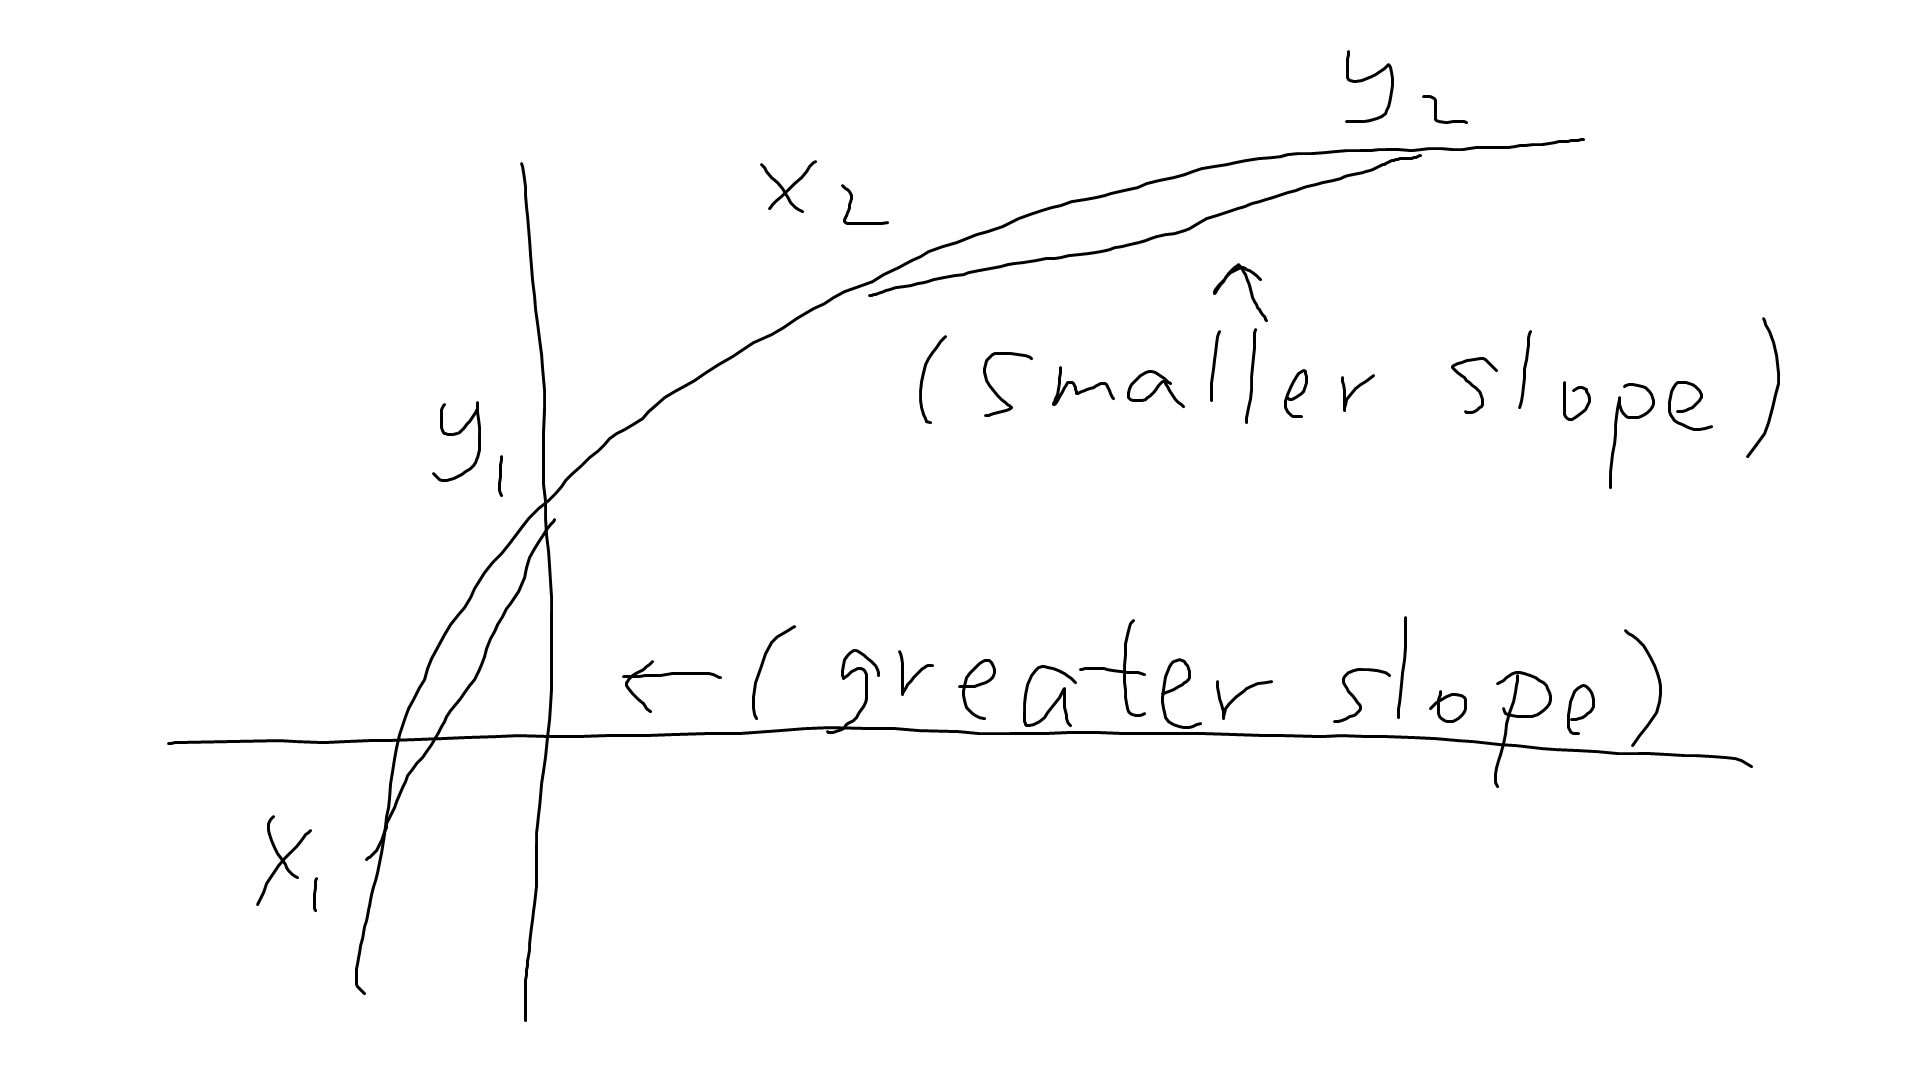
\includegraphics[scale=0.5]{image/SFM_01.png}

\begin{proof}
Let $U$ be concave. It's enough to show the above equation with $y_1 = x_2$ (then apply it twice), so it suffices to show that 
\begin{equation*}
\begin{aligned}
&\frac{U(z) - U(x)}{z-x} \geq \frac{U(y) - U(z)}{y-z} \forall x < z <y\\
\iff &(y-x)U(z) \geq (z-x) U(y) + (y-z)U(x)\\
\iff &\underbrace{(U(z)}_{\geq pU(y)+(1-p)U(x)} \geq \underbrace{\frac{z-x}{y-x}}_{=p \in [0,1]} U(y) + \underbrace{\frac{y-z}{y-x}}_{=1-p} U(x) \ (1.2)
\end{aligned}
\end{equation*}
which holds by concavity.

Conversely, if (1.1) holds then (1.2) also holds which implies concavity.
\end{proof}
\end{prop}

\begin{coro} (1.5)\\
(1) for concave $U$ and $z \in int D(u)$, the interior of regions that $U$ is differentiable, the left and right hand derivatives $$U'_{-}(z) = \lim_{x \to z-} \frac{U(z) - U(x)}{z-x}$$ and $$U'_{+}(z) = \lim_{y \to z+} \frac{U(y) - U(z)}{y-z}$$ exist. Both $U'_+$ and $U'_-$ are decreasing functions and they satisfy $U'_- \geq U'_+$.\\
(2) If $U \in C^2(\R)$, then $U''(x) \leq 0 \forall x$ if and only if $U$ is concave.
\end{coro}

Assume now onward that all utilities are strictly increasing.

Now an agent with wealth $w$ and $C^2$ utility $U$ will accept a contingent claim $X$ provided that $$\E[U(w+X)] > U(w)$$ i.e. his expected utility increases after accepting the contingent claim. If $X$ is asmall, by Taylor expansion we have approximately $U(w) + U'(w) \E[X] + \frac{1}{2} U''(w) \E[X^2] > U(w)$. Recall that $U'(w) > 0$ and $U''(w) < 0$, so the agent benefits from a positive $\E[X]$, and gets a disadvantage from $\E[X^2]$, sort of the variance. This corresponds to the real-life scenario where agents like larger expected gain but dislike larger risk.

The above is balanced if $$\frac{2\E[X]}{\E[X^2]} = -\frac{U''(w)}{U'(w)}$$, the \emph{Arrow-Pratt coefficient(measure) of absolute risk-aversion}.

Similarly, if the proposed gamble is multiplicative instead of additive, i.e. wealth become $w(1+X)$ upon accepting the contingent claim, then the agent will accept it if $\E[U(w(1+X))] > U(w)$. By Taylor expansion we get, if $w>0$, the agent should accept if $$\frac{2\E[X]}{\E[X^2]} \geq -\frac{wU''(w)}{U'(w)}$$, the \emph{Arrow-Pratt coefficient of relative risk-aversion}.

Check by substitution how these relate to the examples (1) and (2) in (1.3), which explains the name of them (CARA and CRRA).

\subsection{Reservation and marginal prices}
If an agent can choose claims from an admissible set $A$, he will try to achieve $\sup_{X \in A} \E[U(X)]$.

Suppose the sup is attained in $X^* \in A$ and suppose that $A$ is an affine space of the form $A = X^* + V$ where $V$ is a vector space. Then, $\forall \xi \in V$, $t \in \R$, $\E[U(X^*)] \geq \E[U(X^*+t\xi)]$ and differentiating w.r.t. $t$ gives $$ \E[U'(X^*) \xi] =0 \ (1.3)$$ for all $\xi \in V$.

\iffalse
\begin{equation*}
\begin{aligned}

\end{aligned}
\end{equation*}
\fi



\end{document}
